\chapter{評価}
\label{chap:evaluation}

計測用のプログラムとして、与えられた整数$n$に対して$n$番目のフィボナッチ数を返す関数$fib(n)$を
C言語で実装した。
実装は、再帰呼び出しによる実装、ローカル変数を用いた実装およびヒープを用いた実装の3種類を用意した。

\begin{itembox}[l]{再帰呼び出しによる実装}
  \begin{verbatim}
    int fib(int n) {
      if (n <= 1) return 1;
      return fib(n - 1) + fib(n - 2);
    }
  \end{verbatim}
\end{itembox}

\begin{itembox}[l]{ローカル変数を用いた実装}
  \begin{verbatim}
    int fib(int n) {
      if (n <= 1) return 1;

      int arr[n];
      arr[0] = arr[1] = 1;
      for (int i = 2; i < n; i++)
        arr[i] = arr[i - 1] + arr[i - 2];

      return arr[n];
    }
  \end{verbatim}
\end{itembox}

\begin{itembox}[l]{ヒープを用いた実装}
  \begin{verbatim}
    int fib(int n) {
    }
  \end{verbatim}
\end{itembox}

これらの関数をLLVM/Clang 7.0でWebAssemblyモジュールとしてコンパイルして得られたバイナリを、
\ref{chap:implementation}で述べたESP32用プログラムを用いてそれぞれ実行した。
また、これらの関数を\verb|関数|を直接呼び出すプログラムを既存のESP32ツールチェインにより
コンパイルし、それぞれ実行した。

また、それぞれの実行は引数\verb|n|を1から15まで変化させ、実行速度およびメモリフットプリントの
変化を計測した。
また、それぞれのプログラムサイズを計測した。

\section{実行速度}

実行速度は、FreeRTOSの\verb|vTaskGetRunTimeStats|を用いて計測した。

ネイティブ実行に対するWebAssemblyバイナリの実行速度について、再帰呼び出しによる実装では約3倍、
ローカル変数を用いた実装では約10倍、ヒープを用いた実装では約5倍だった。
引数nを1から15まで変化させた時の、実行速度の推移を\ref{fig:exec_time}に示す。

\begin{figure}[htbp]
  \caption{実行速度の推移とその比較}
  \label{fig:exec_time}
  \begin{center}
    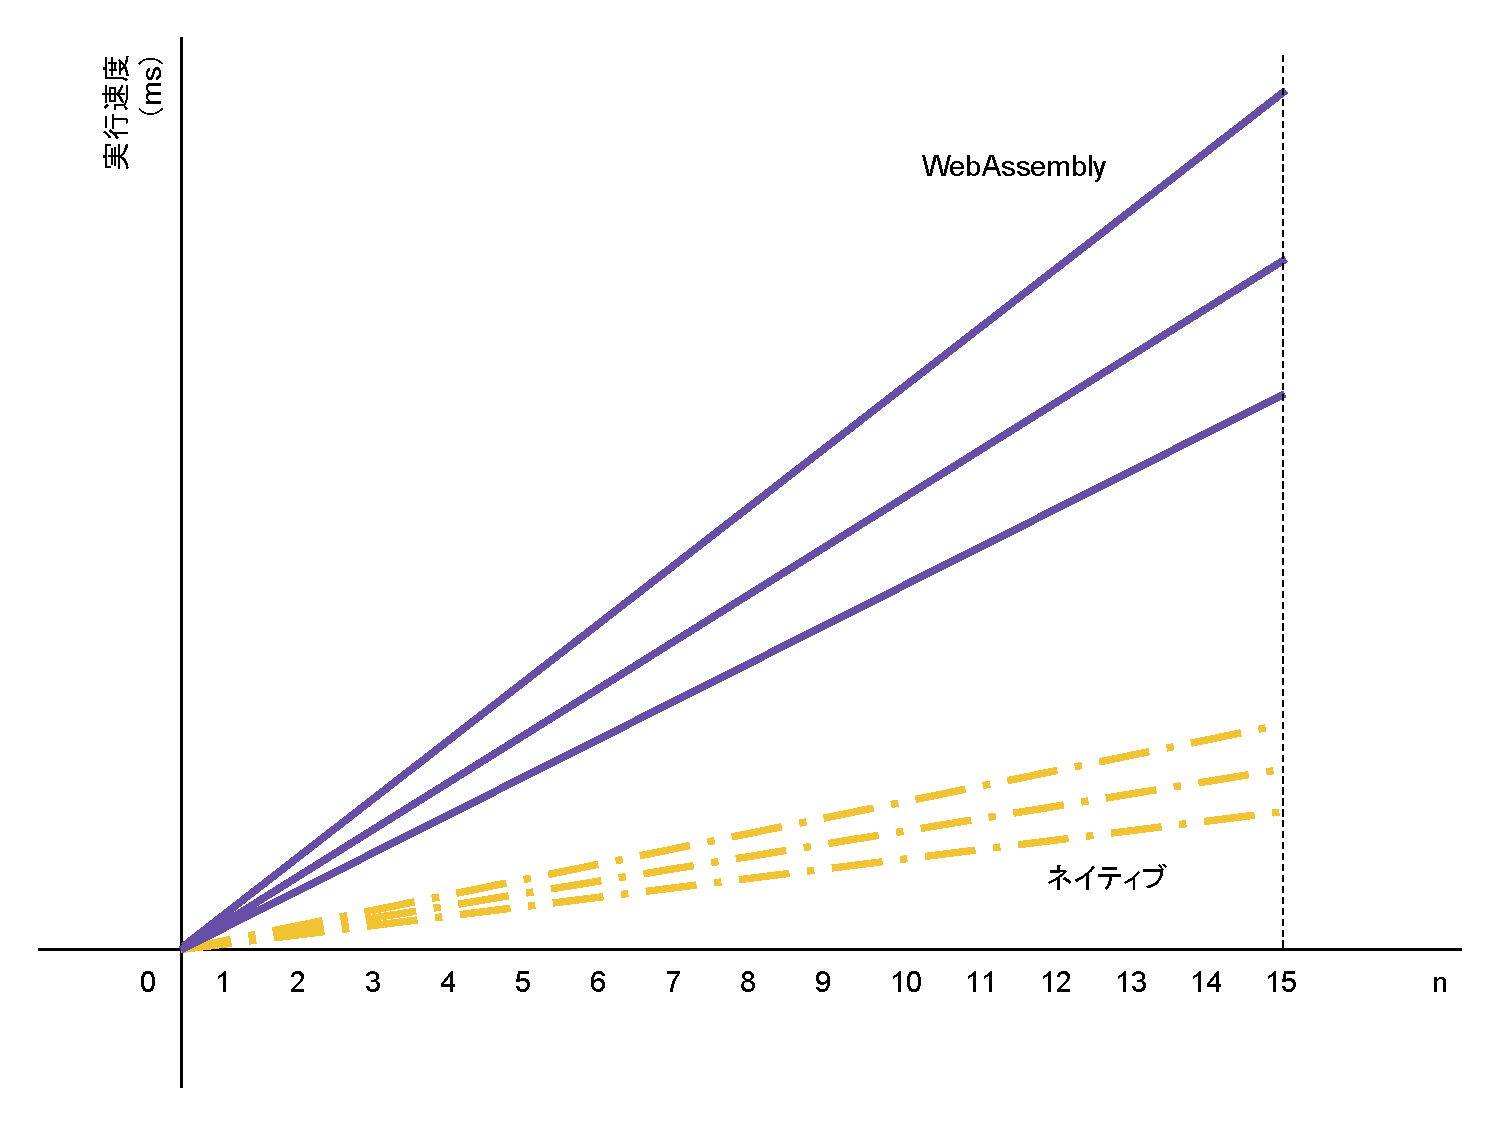
\includegraphics[bb=0 0 800 600,width=12cm]{img/exec_time.pdf}
  \end{center}
\end{figure}

\section{メモリ使用量}

それぞれの実装方法について、コンパイル後のプログラムは、WebAssemblyを用いた場合が
ネイティブ実行を用いた場合に比べて約3倍のサイズとなった。

コンパイル後の全体のプログラムサイズの比較を\ref{tb:program_size}に示す。

\begin{table}[]
  \caption{プログラムサイズ}
  \label{tb:program_size}
  \begin{center}
    \begin{tabular}{|l|l|l|l|}
      \hline
      & 再帰 & ローカル変数 & ヒープ \\ \hline
      WebAssembly & 300 KB & 350 KB & 325 KB \\ \hline
      ネイティブ & 100 KB & 101 KB & 99 KB \\ \hline
    \end{tabular}
  \end{center}
\end{table}

実行中のメモリフットプリントは、〜により計測した。
ネイティブ実行に対するWebAssemblyバイナリの実行速度について、それぞれの実装方法においておおよそ
3倍のオーバーヘッドがあった。
引数nを1から15まで変化させた時の、メモリフットプリントの推移を\ref{fig:heap_size}に示す。

\begin{figure}[htbp]
  \caption{メモリフットプリントの推移とその比較}
  \label{fig:heap_size}
  \begin{center}
    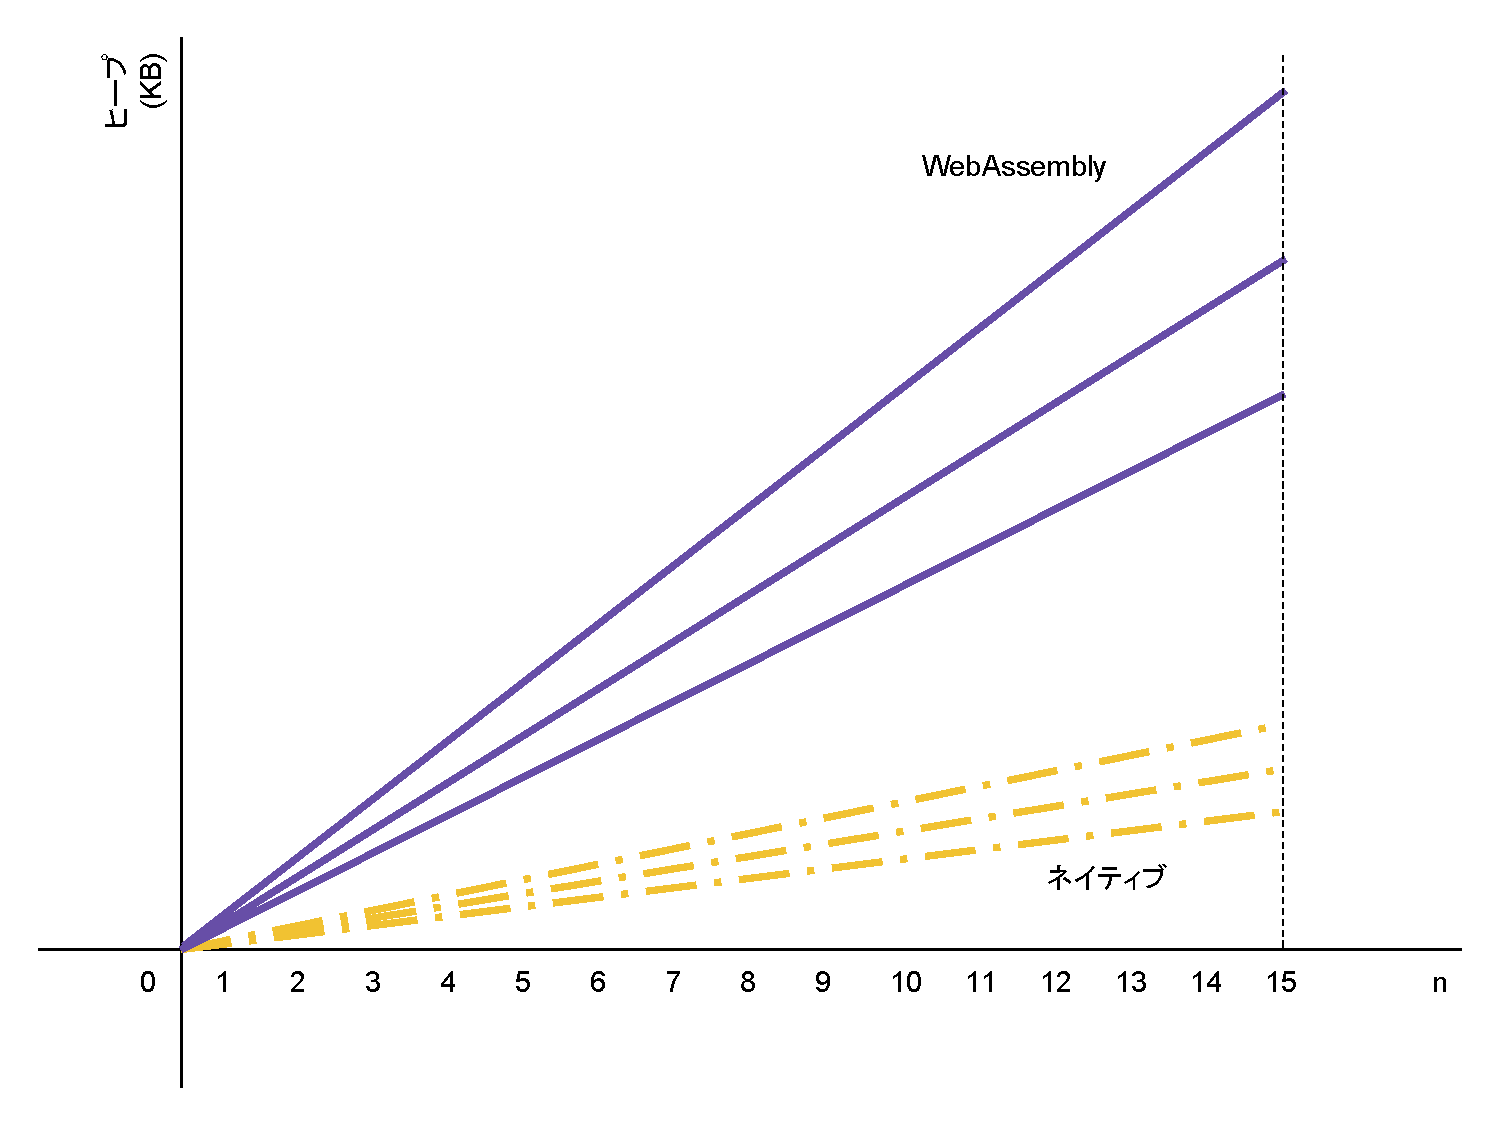
\includegraphics[bb=0 0 800 600,width=12cm]{img/heap_size.pdf}
  \end{center}
\end{figure}
